% Thesis Proposal

\documentclass[11pt,english]{article}
\usepackage{graphicx}
\usepackage[T1]{fontenc}
\usepackage[latin9]{inputenc}
\usepackage{float}
\usepackage{color}
\usepackage{amsmath,array}
\usepackage{caption}
\usepackage{units}
\usepackage{verbatim}
\usepackage{geometry,subcaption}
\geometry{verbose,tmargin=1in,bmargin=1in,lmargin=1in,rmargin=1in}
\begin{document}

\title{Outline of the second stabilization paper}

\author{Sili Deng}
\maketitle

%============================================================================
\section{Introduction}

\begin{itemize}
  \item Nonpremixed lifted flame stabilization at nonautoignitive conditions.
  \item In engineering applications, power engines run at elevated temperature and pressure conditions.  Autoignition and NTC phenomenon are present.
  \item Review Krisman and the first paper.
  \item Objectives of the present paper.
  \begin{itemize}
    \item Residence time effects.
    \item Detailed analysis of the multibrachial structure.  Demonstrate the coupling between autoignition and flame propagation.
  \end{itemize}
\end{itemize}

%============================================================================
\section{Computational Details}


%============================================================================
\section{Residence Time Effects}

Case description.  $900$ K, $2.4$, $3.2$, and $8.0$ m/s.  (Table with computational specifications?) 

\subsection{Thermal and Chemical Structure}
\begin{itemize}
  \item HRR profiles.  Fig.~\ref{fig:HRR_velocity}
    \begin{figure}[t]
      \centering
      \scriptsize
      %\vspace{-0.1in}
      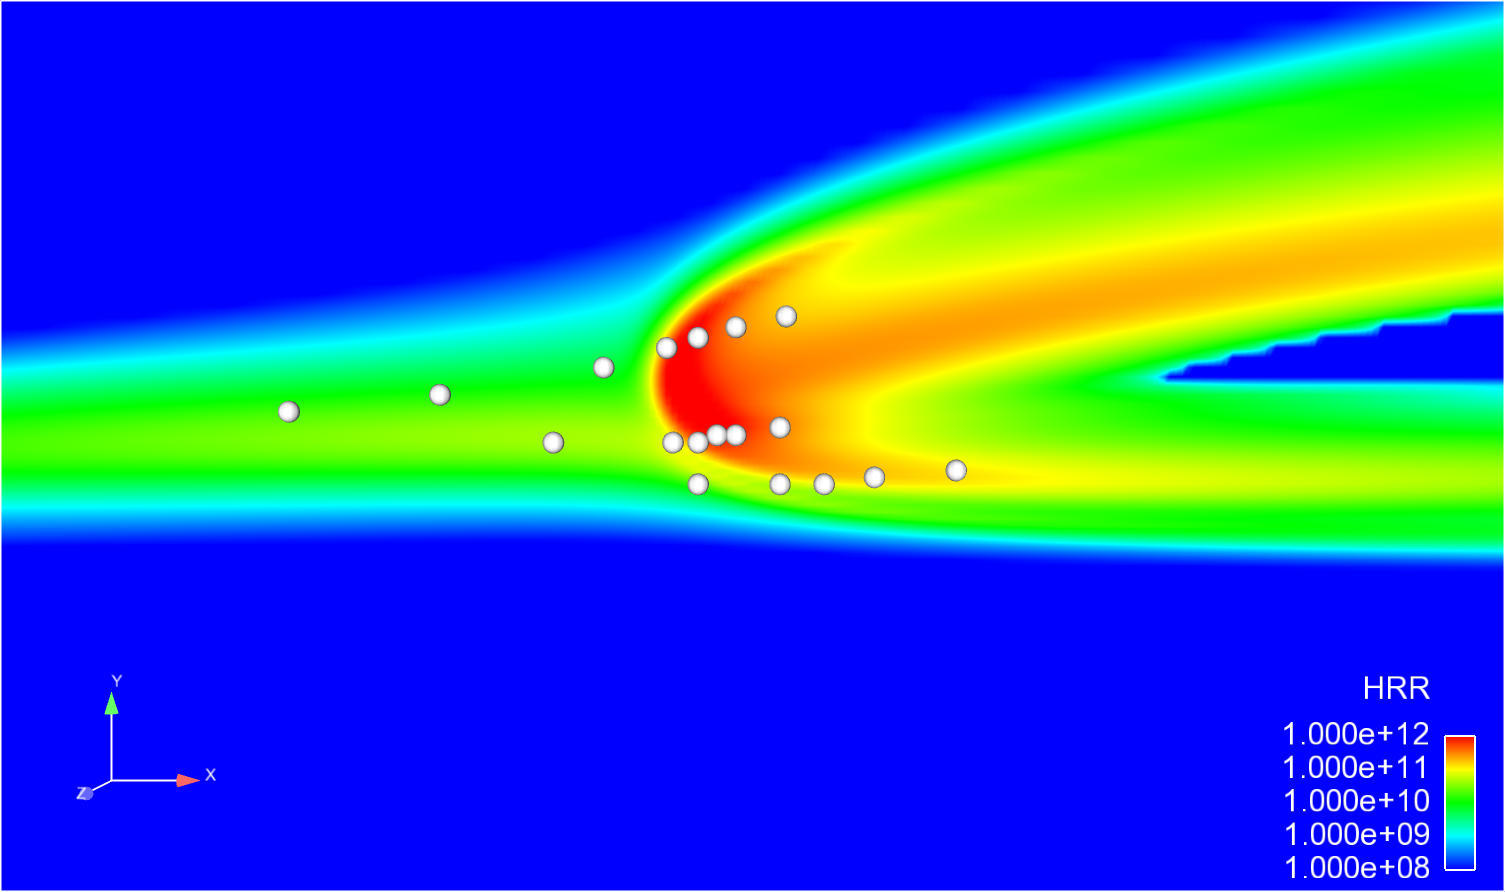
\includegraphics[width=0.3\textwidth]{HRR_2_4.png}
      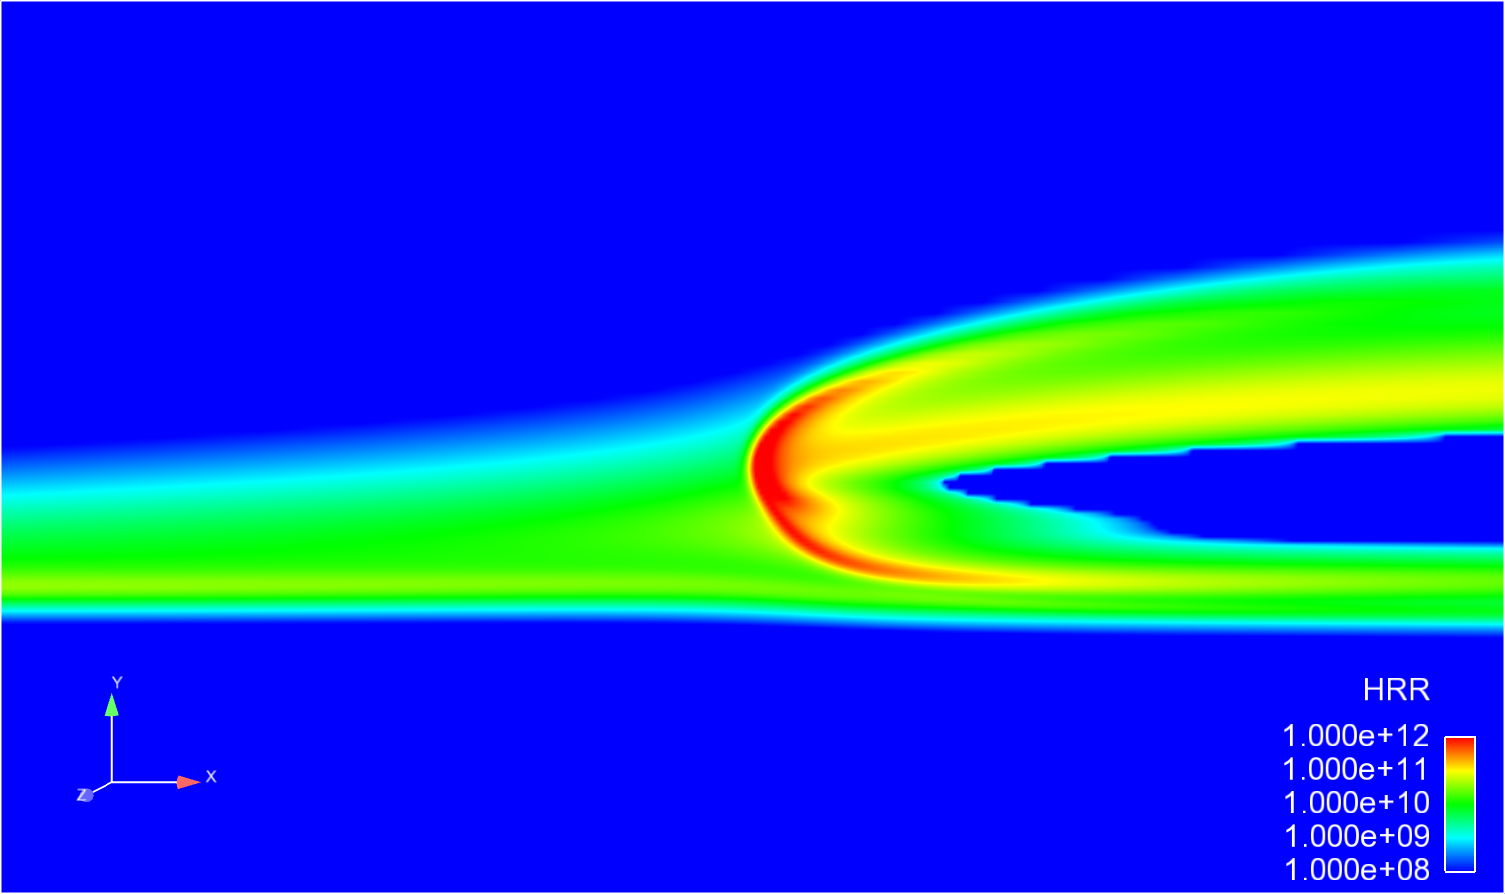
\includegraphics[width=0.3\textwidth]{HRR_3_2.png}
      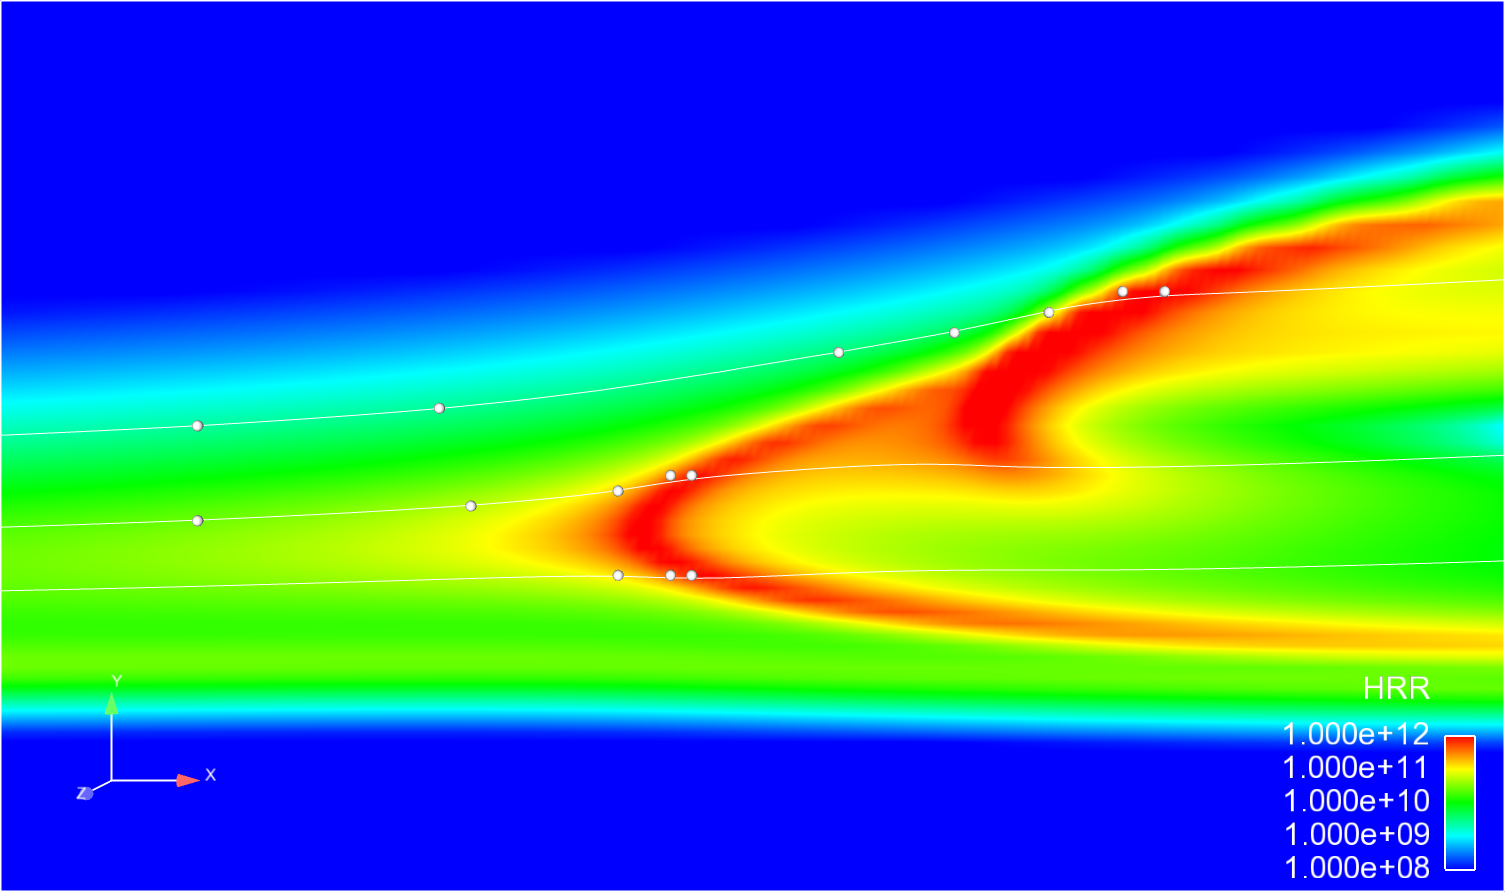
\includegraphics[width=0.3\textwidth]{HRR_8_0.png}
      \normalsize
      %\vspace{-0.1in}
      \caption{$2.4$, $3.2$, and $8.0$ m/s.}
      \label{fig:HRR_velocity}
    \end{figure} 
  \item CEMA results showing the dominant reactions and combustion mode.
\end{itemize}

\subsection{Stabilization Mechanism}
\begin{itemize}
  \item LFA-CFD comparison to demonstrate the system response and the stabilization mechanism.  Fig.~\ref{fig:LFA_velocity}
\end{itemize}
\begin{figure}[t]
      \centering
      \scriptsize
      %\vspace{-0.1in}
      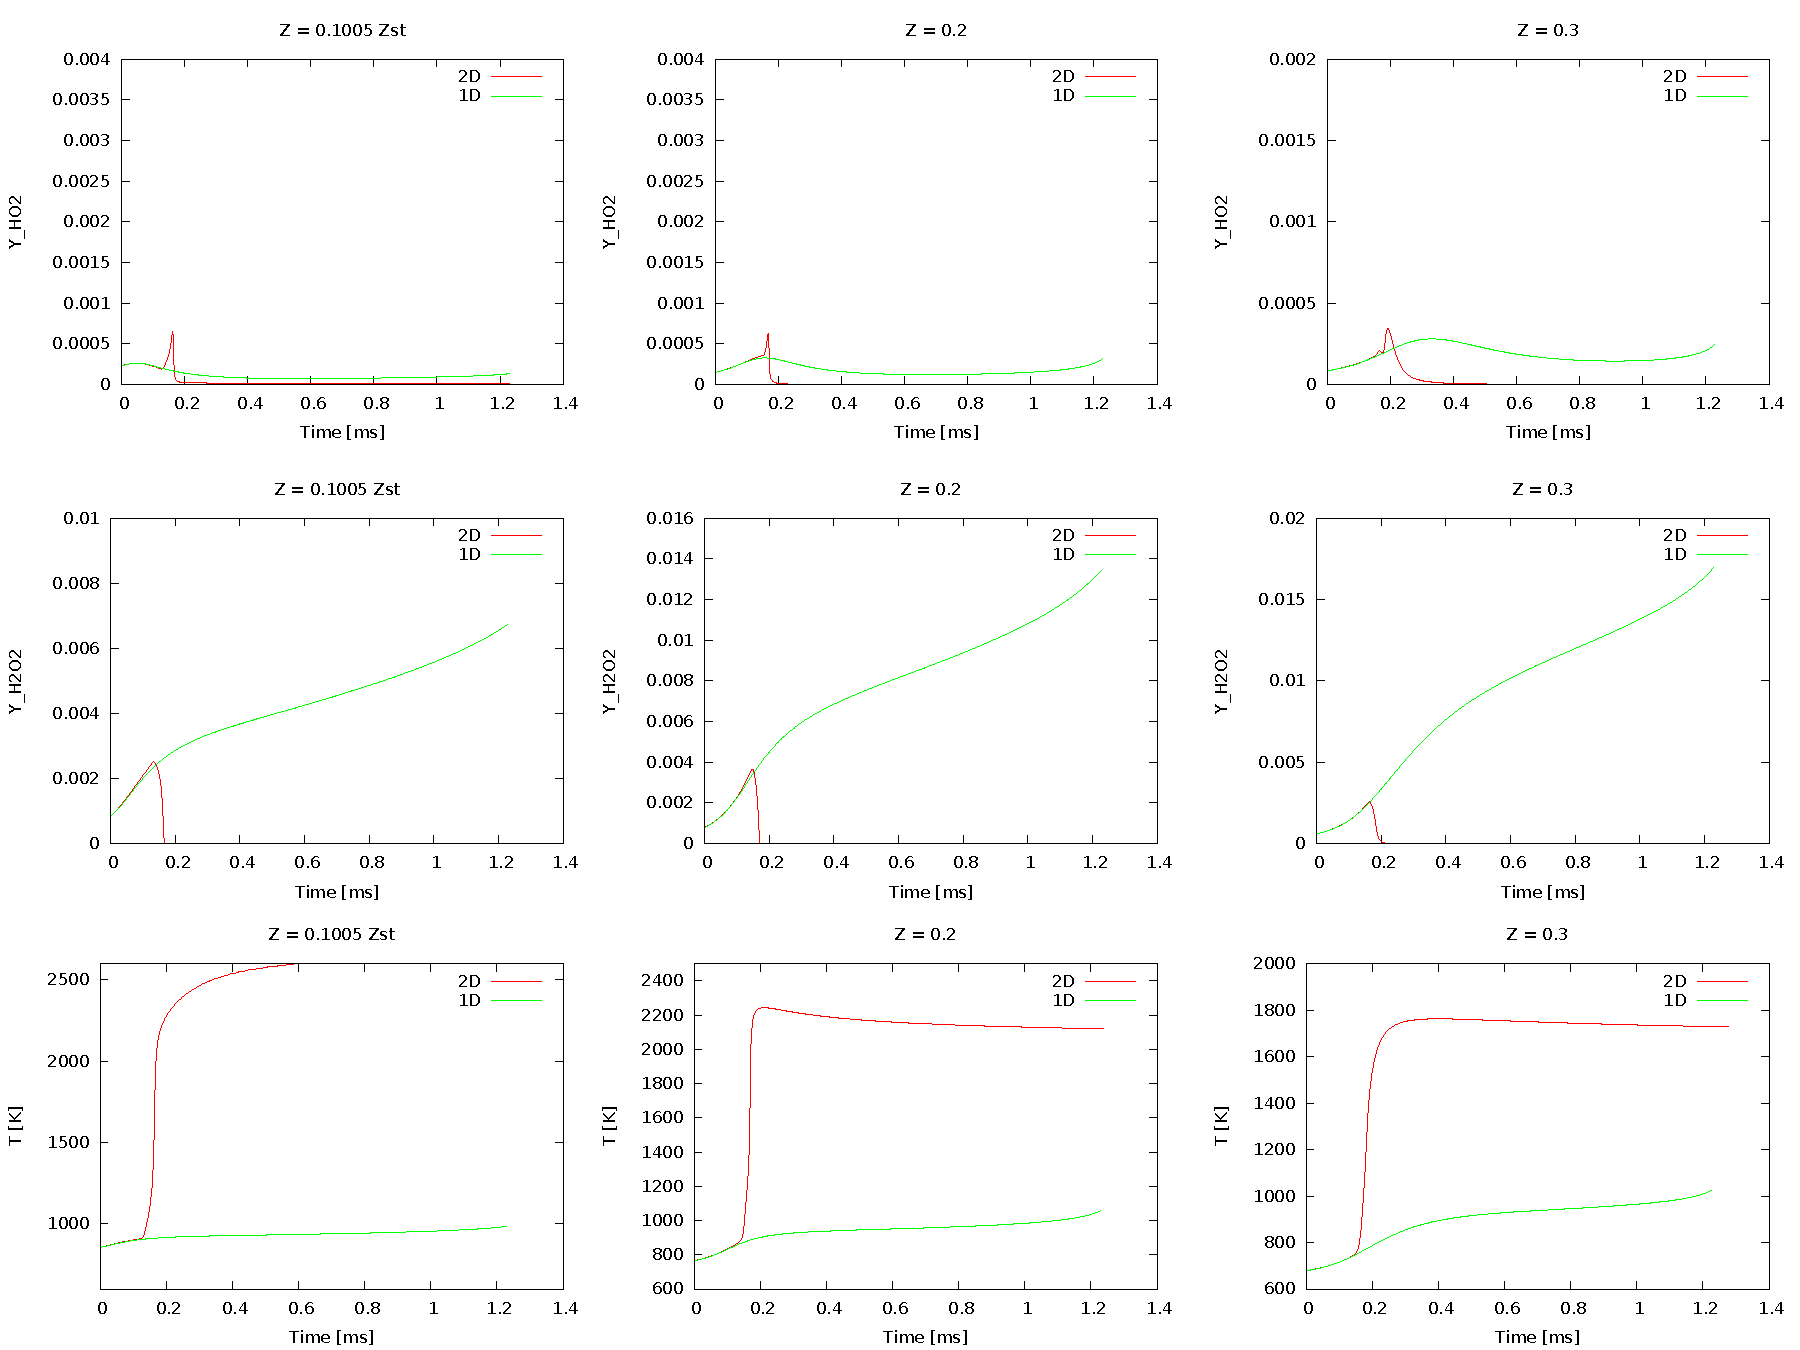
\includegraphics[width=0.3\textwidth]{2_4_profile_time.pdf}
      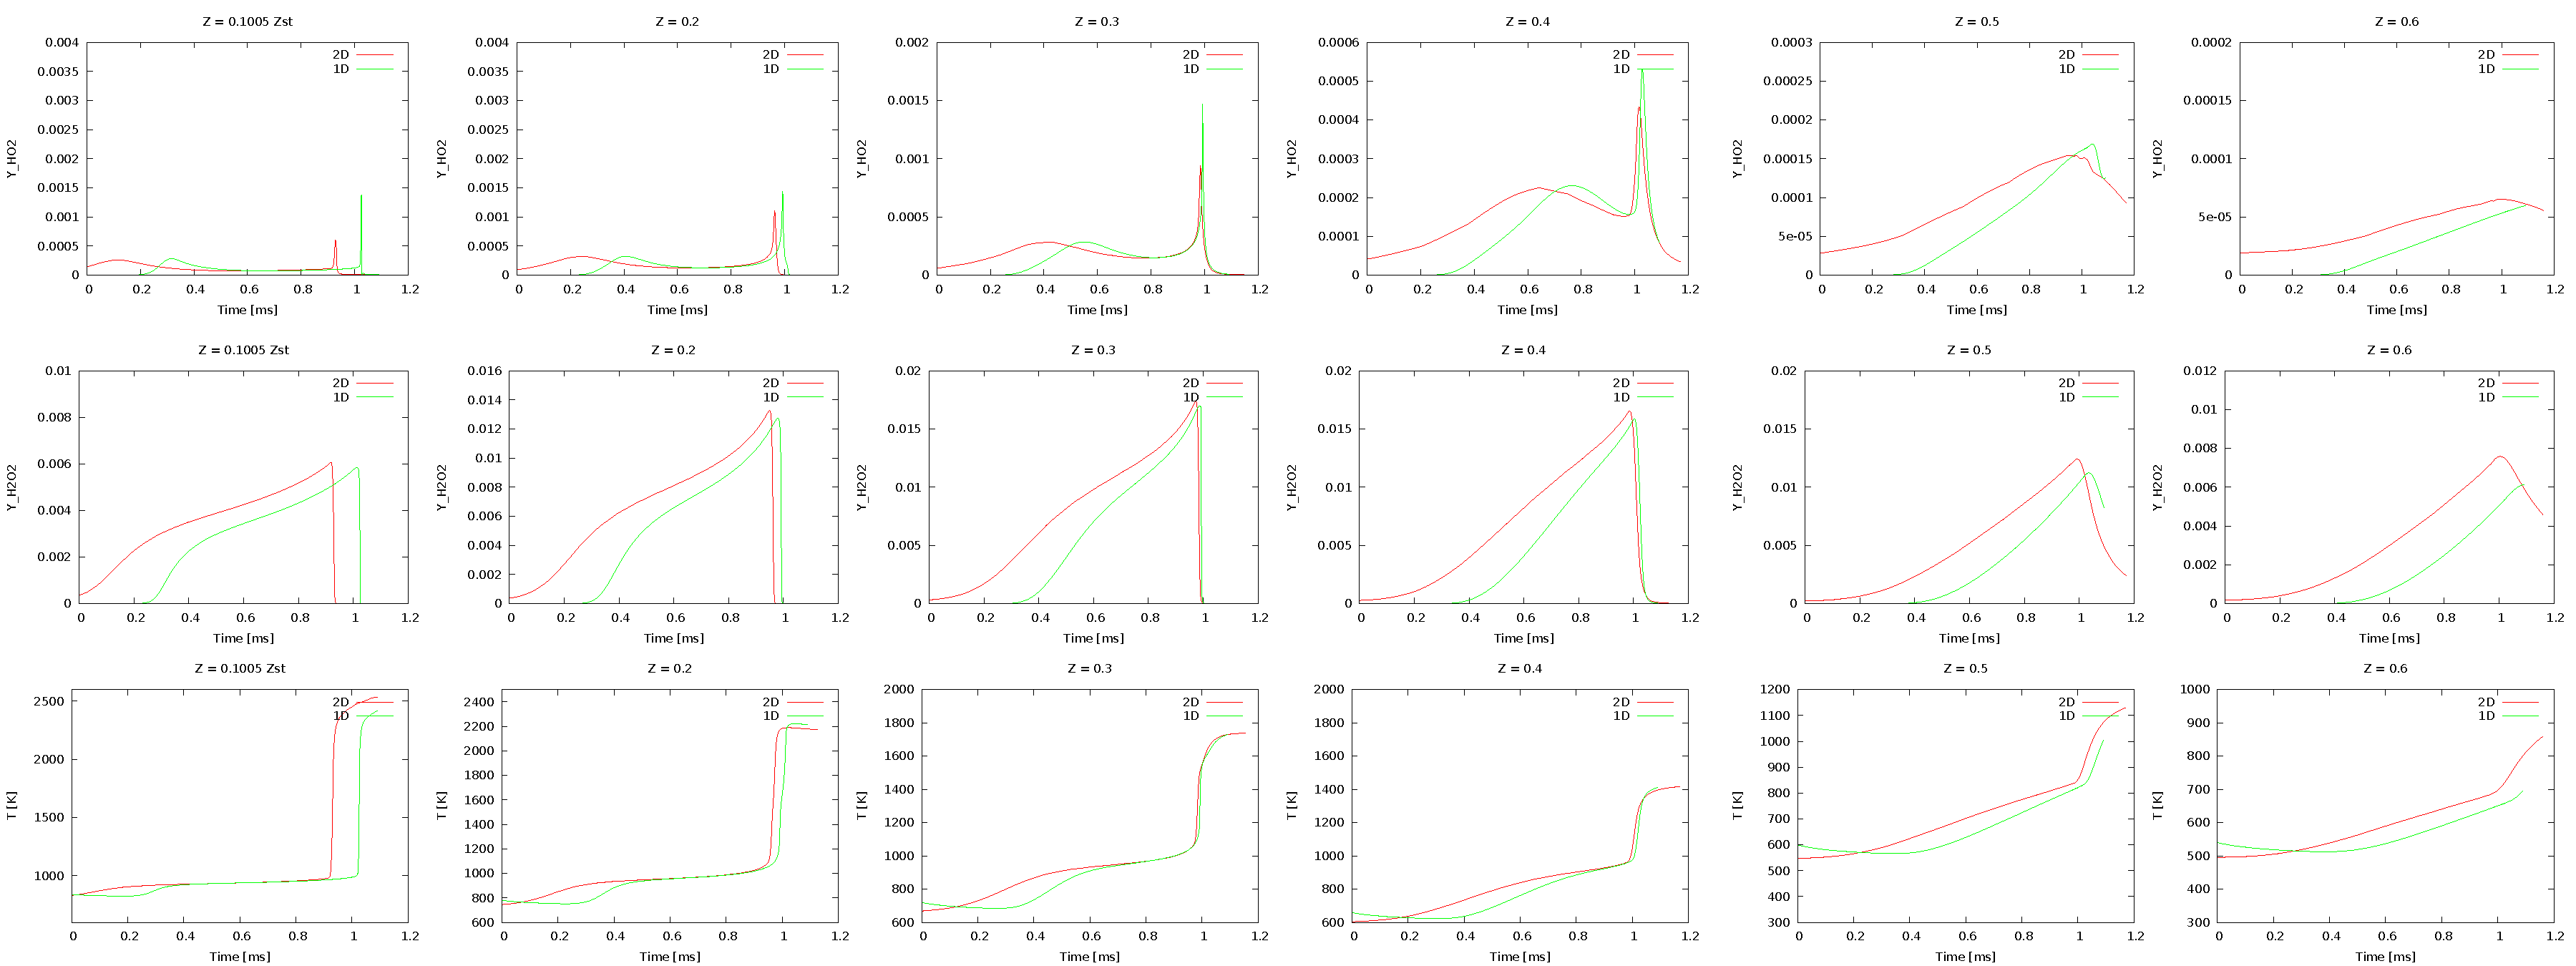
\includegraphics[trim = 0 0 305mm 0, clip, width=0.3\textwidth]{900_profile_time.pdf}
      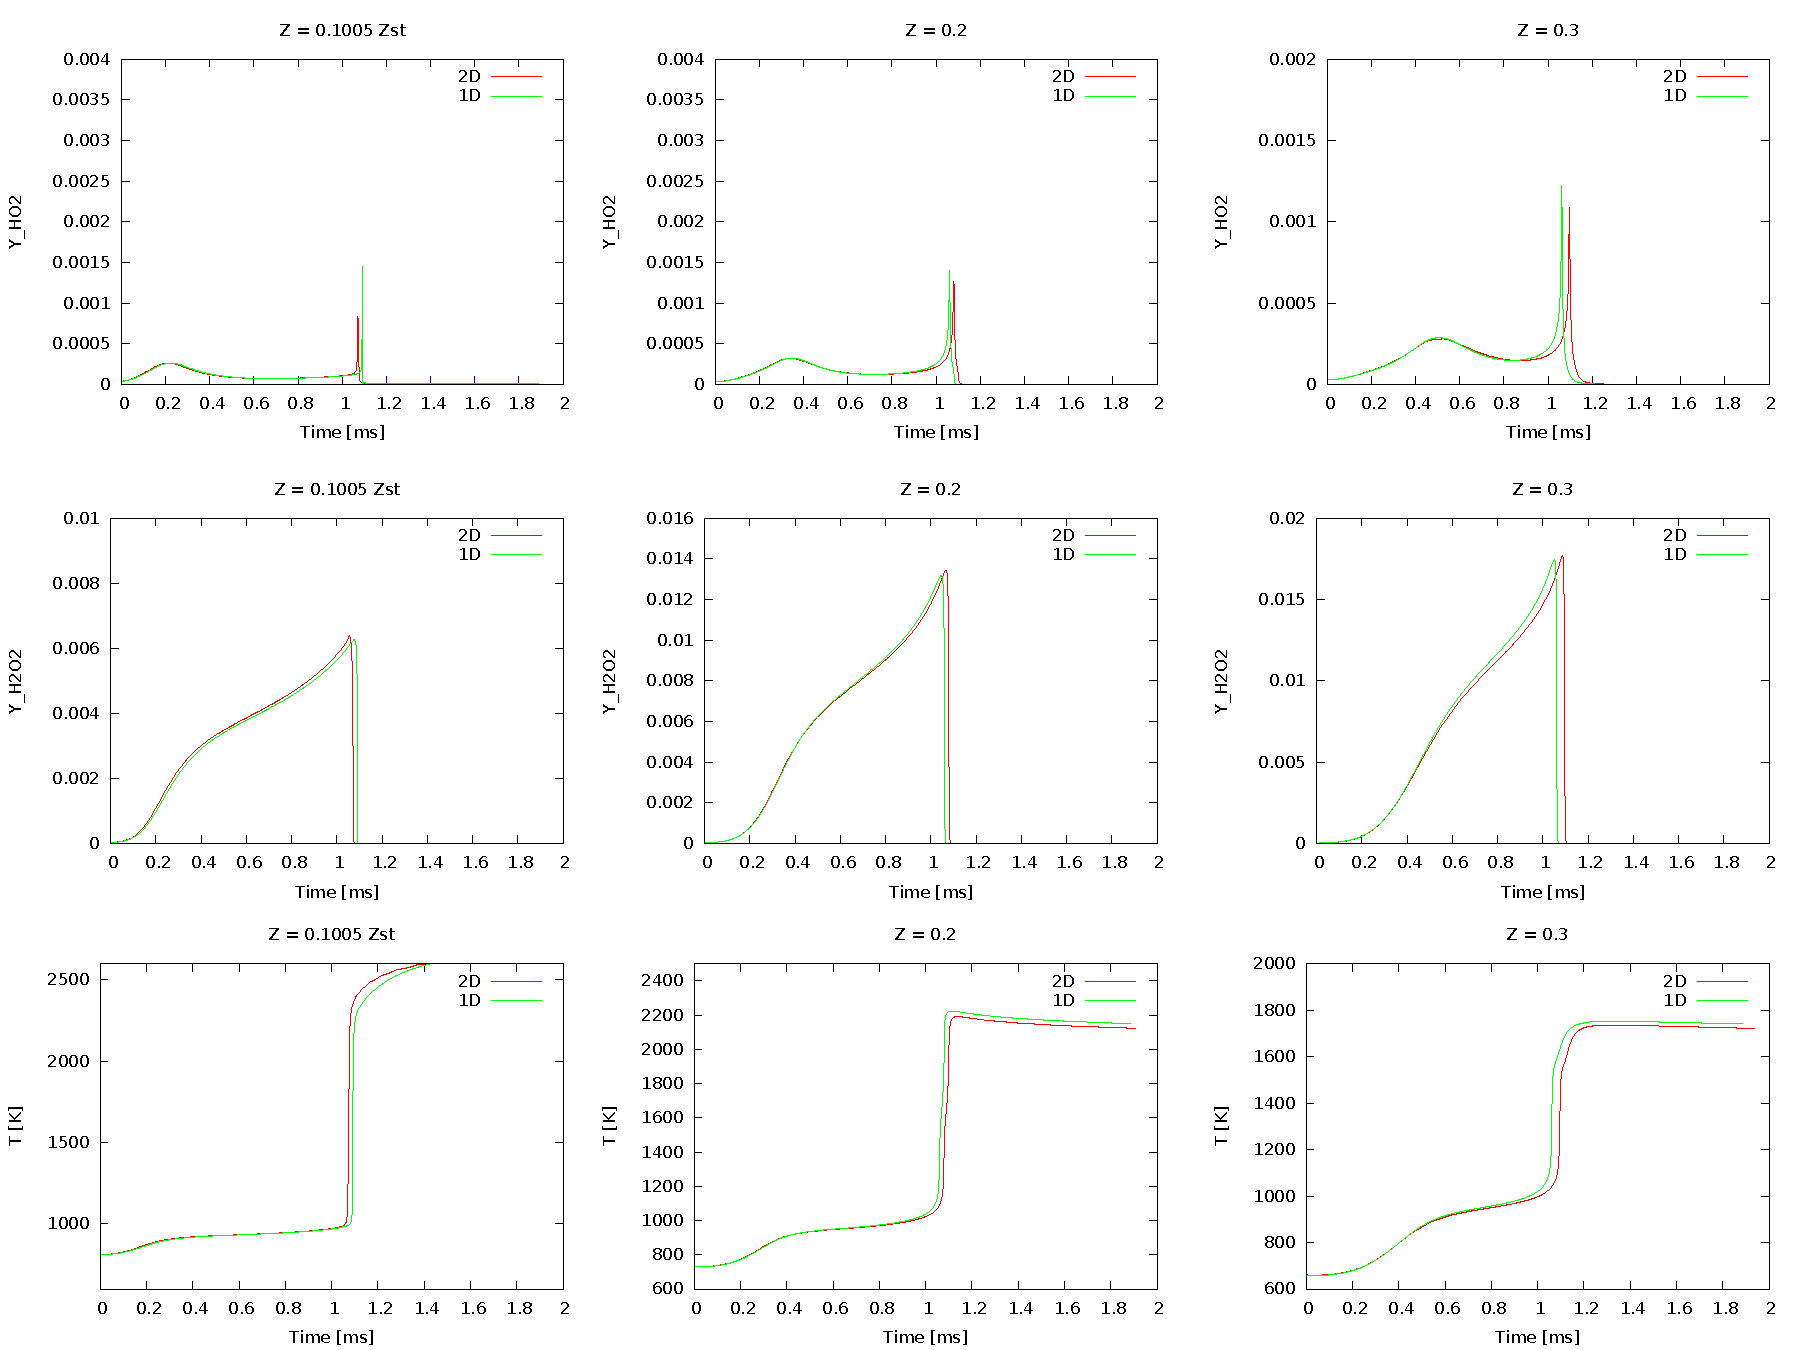
\includegraphics[width=0.3\textwidth]{8_0_profile_time.pdf}
      \normalsize
      %\vspace{-0.1in}
      \caption{$2.4$, $3.2$, and $8.0$ m/s.}
      \label{fig:LFA_velocity}
    \end{figure} 

\subsection{Stabilization Regime Diagram}
With dimensions.  T and V.

%============================================================================
\section{Autoignition-Flame-Coupling}
Case description.  $800$ K, with and without dilution.  (Table with computational specifications?)

\subsection{Thermal and Chemical Structure}
\begin{itemize}
  \item HRR profiles.  Fig.~\ref{fig:HRR_dilution}
    \begin{figure}[t]
      \centering
      \scriptsize
      %\vspace{-0.1in}
      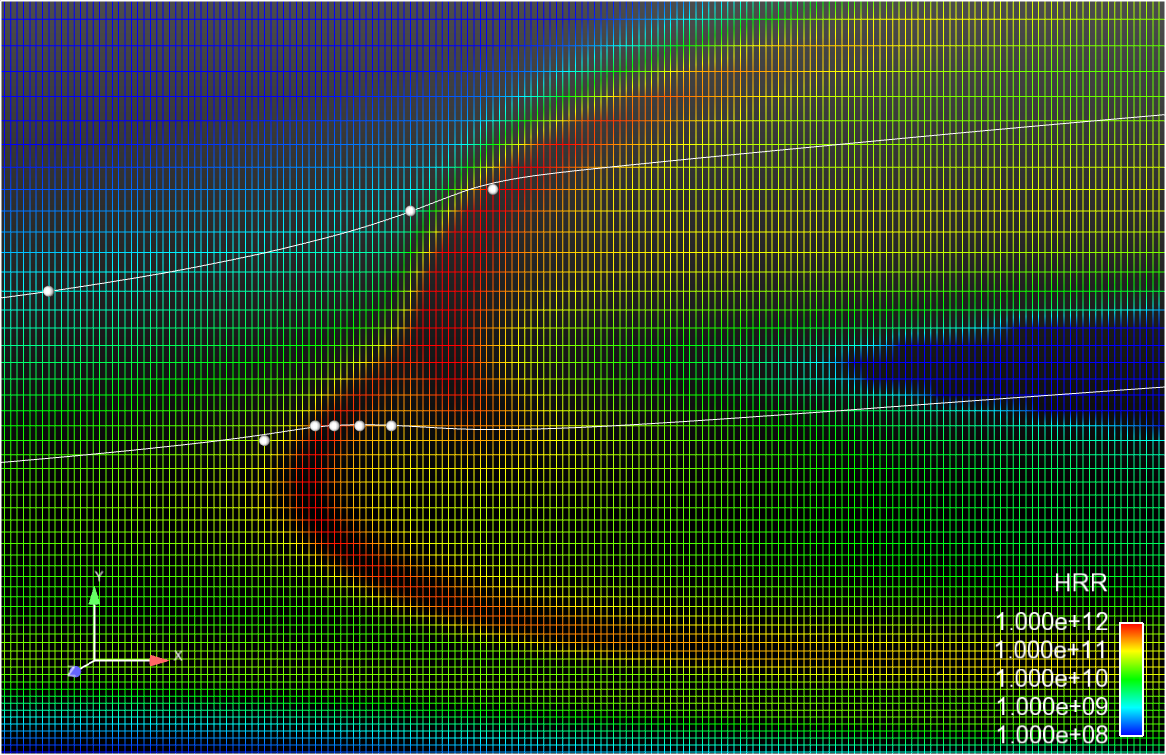
\includegraphics[width=0.5\textwidth]{HRR_nodil.png}
      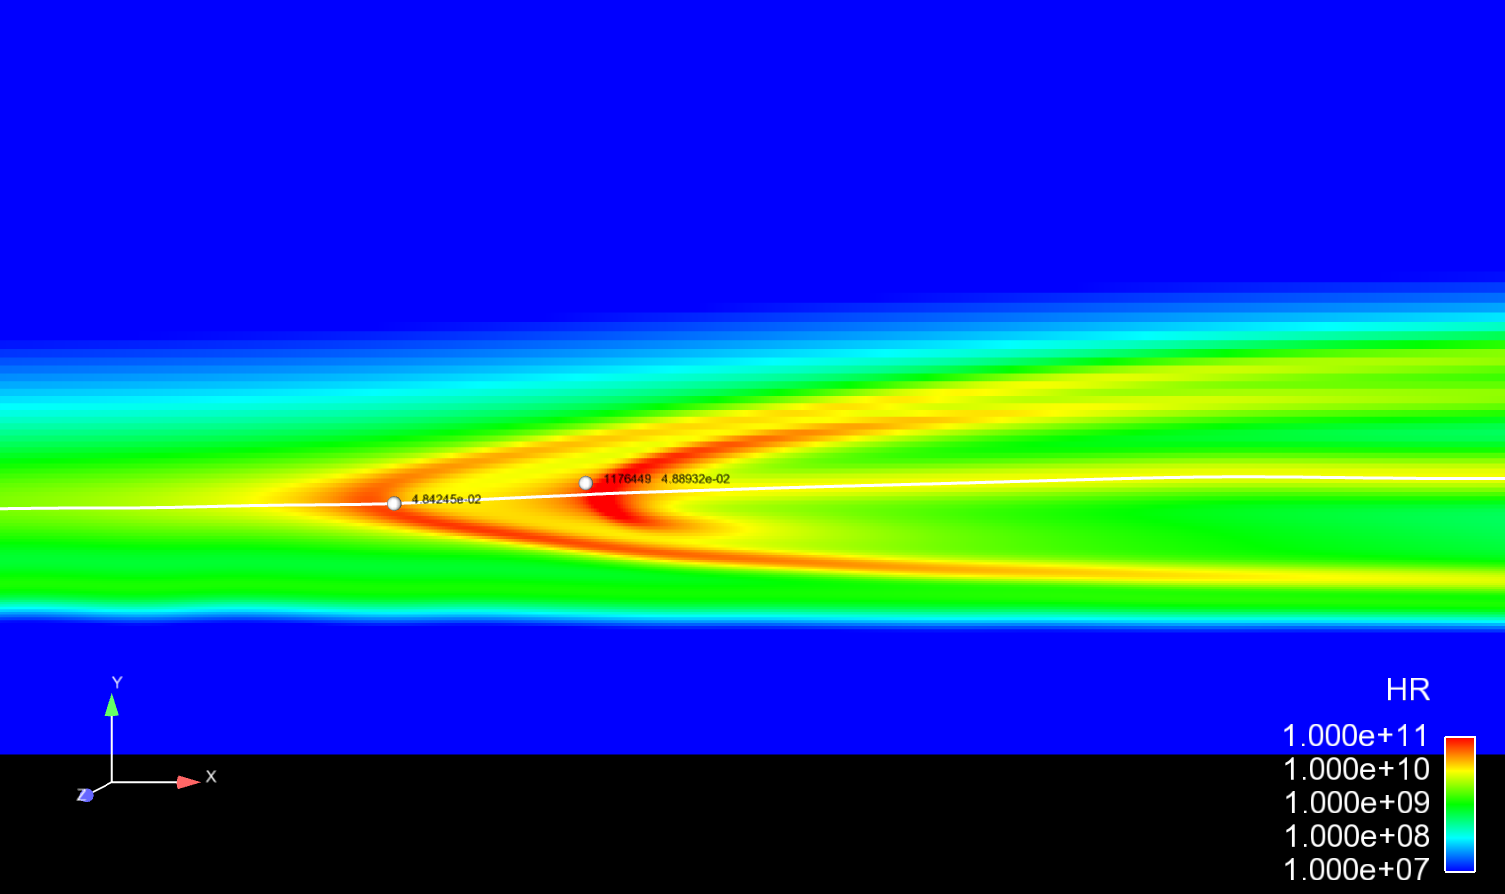
\includegraphics[width=0.5\textwidth]{HRR_dilution.png}
      \normalsize
      %\vspace{-0.1in}
      \caption{With and without dilution.}
      \label{fig:HRR_dilution}
    \end{figure} 
  \item CEMA results showing the dominant reactions and combustion mode.
\end{itemize}

\subsection{Stabilization Mechanism}
\begin{itemize}
  \item 0-1-2D comparison to demonstrate the system response and the stabilization mechanism.  Fig.~\ref{fig:LFA_800_nodil} and Fig.~\cite{fig:LFA_800_dilution}.
\end{itemize}
\begin{figure}[t]
      \centering
      \scriptsize
      %\vspace{-0.1in}
      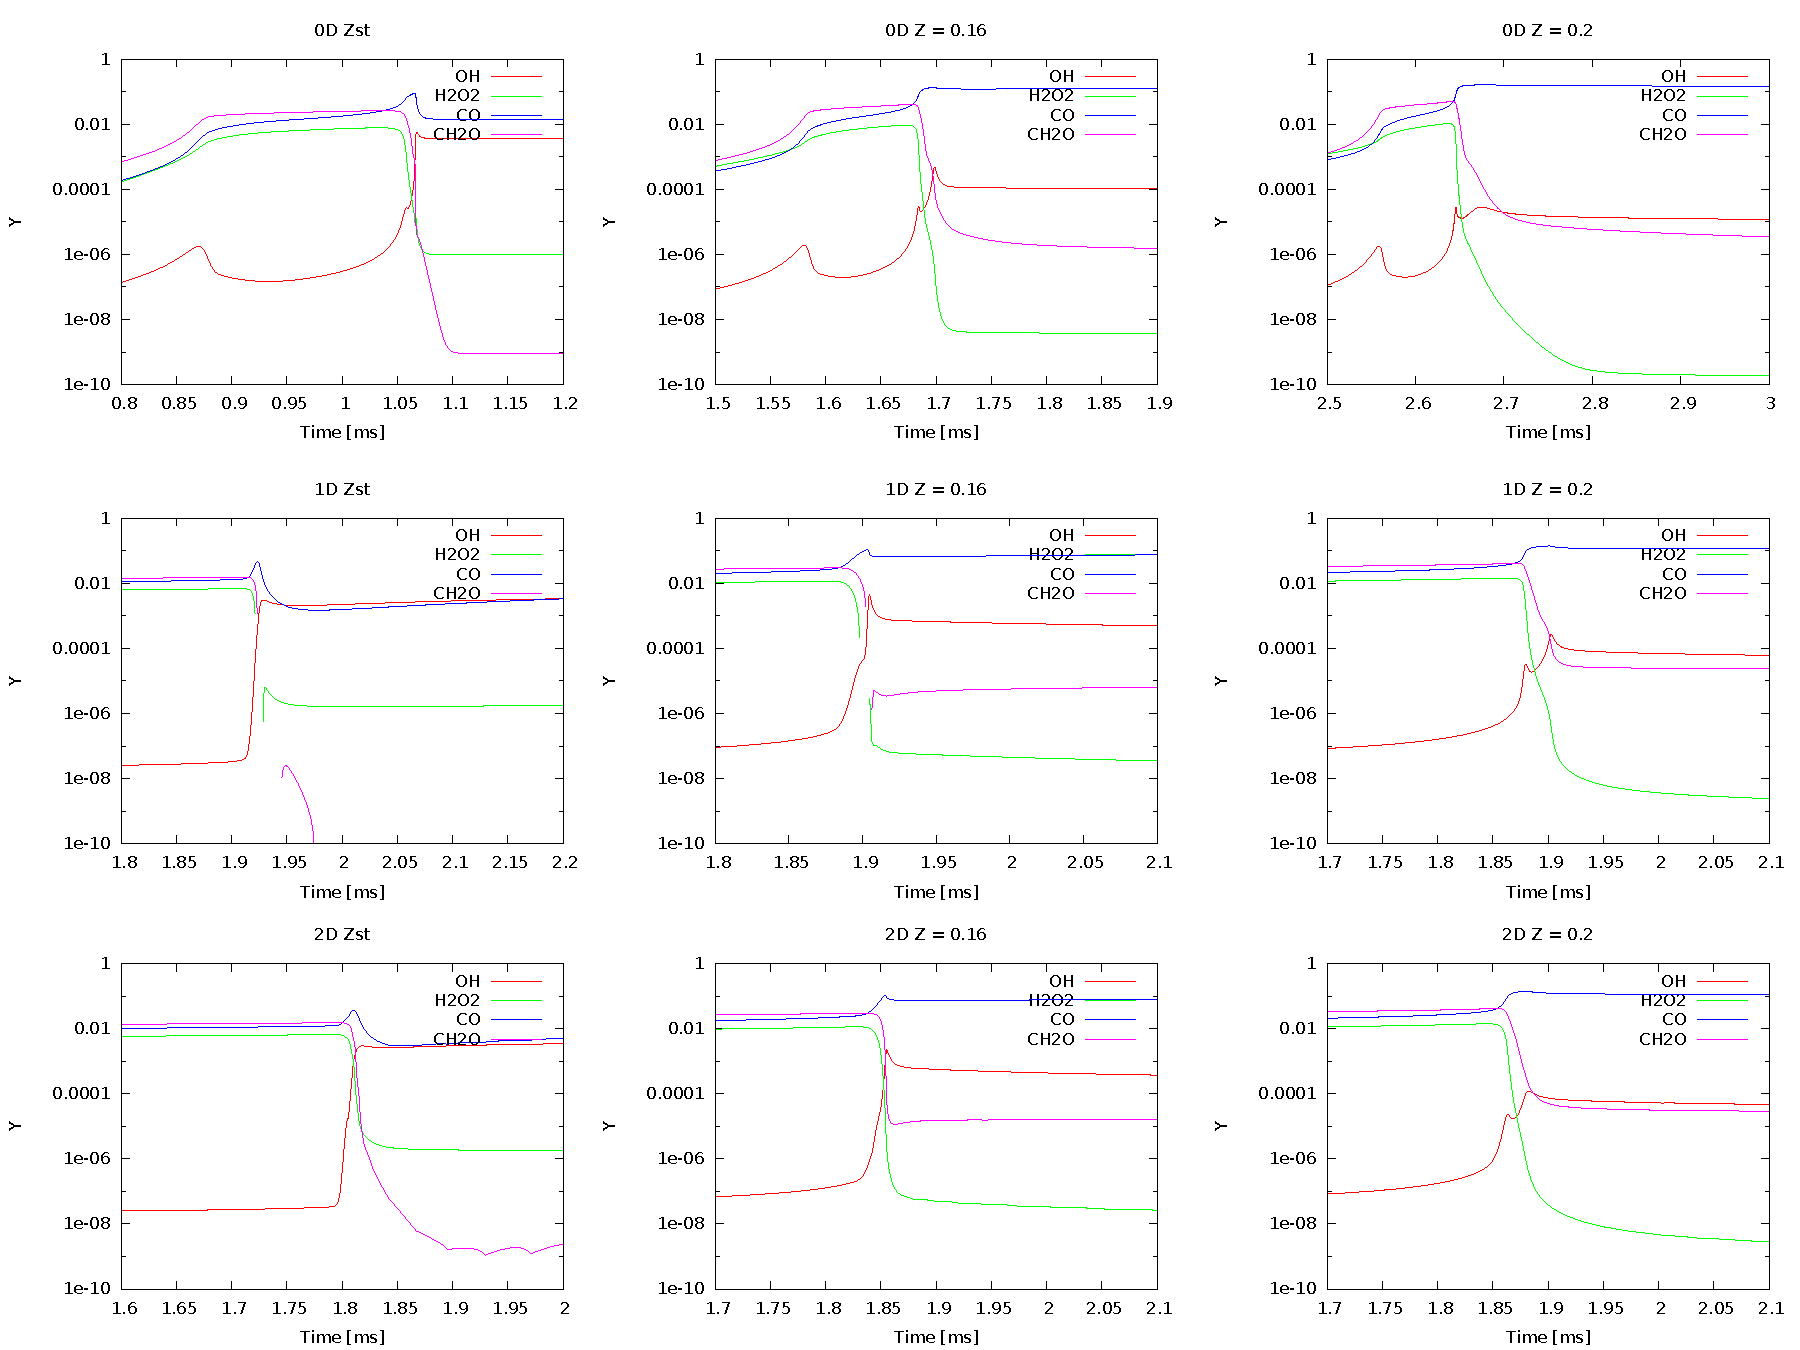
\includegraphics[width=1.0\textwidth]{800_nodil_012D.pdf}
      \normalsize
      %\vspace{-0.1in}
      \caption{Without dilution.}
      \label{fig:LFA_800_nodil}
    \end{figure} 

\begin{figure}[t]
      \centering
      \scriptsize
      %\vspace{-0.1in}
      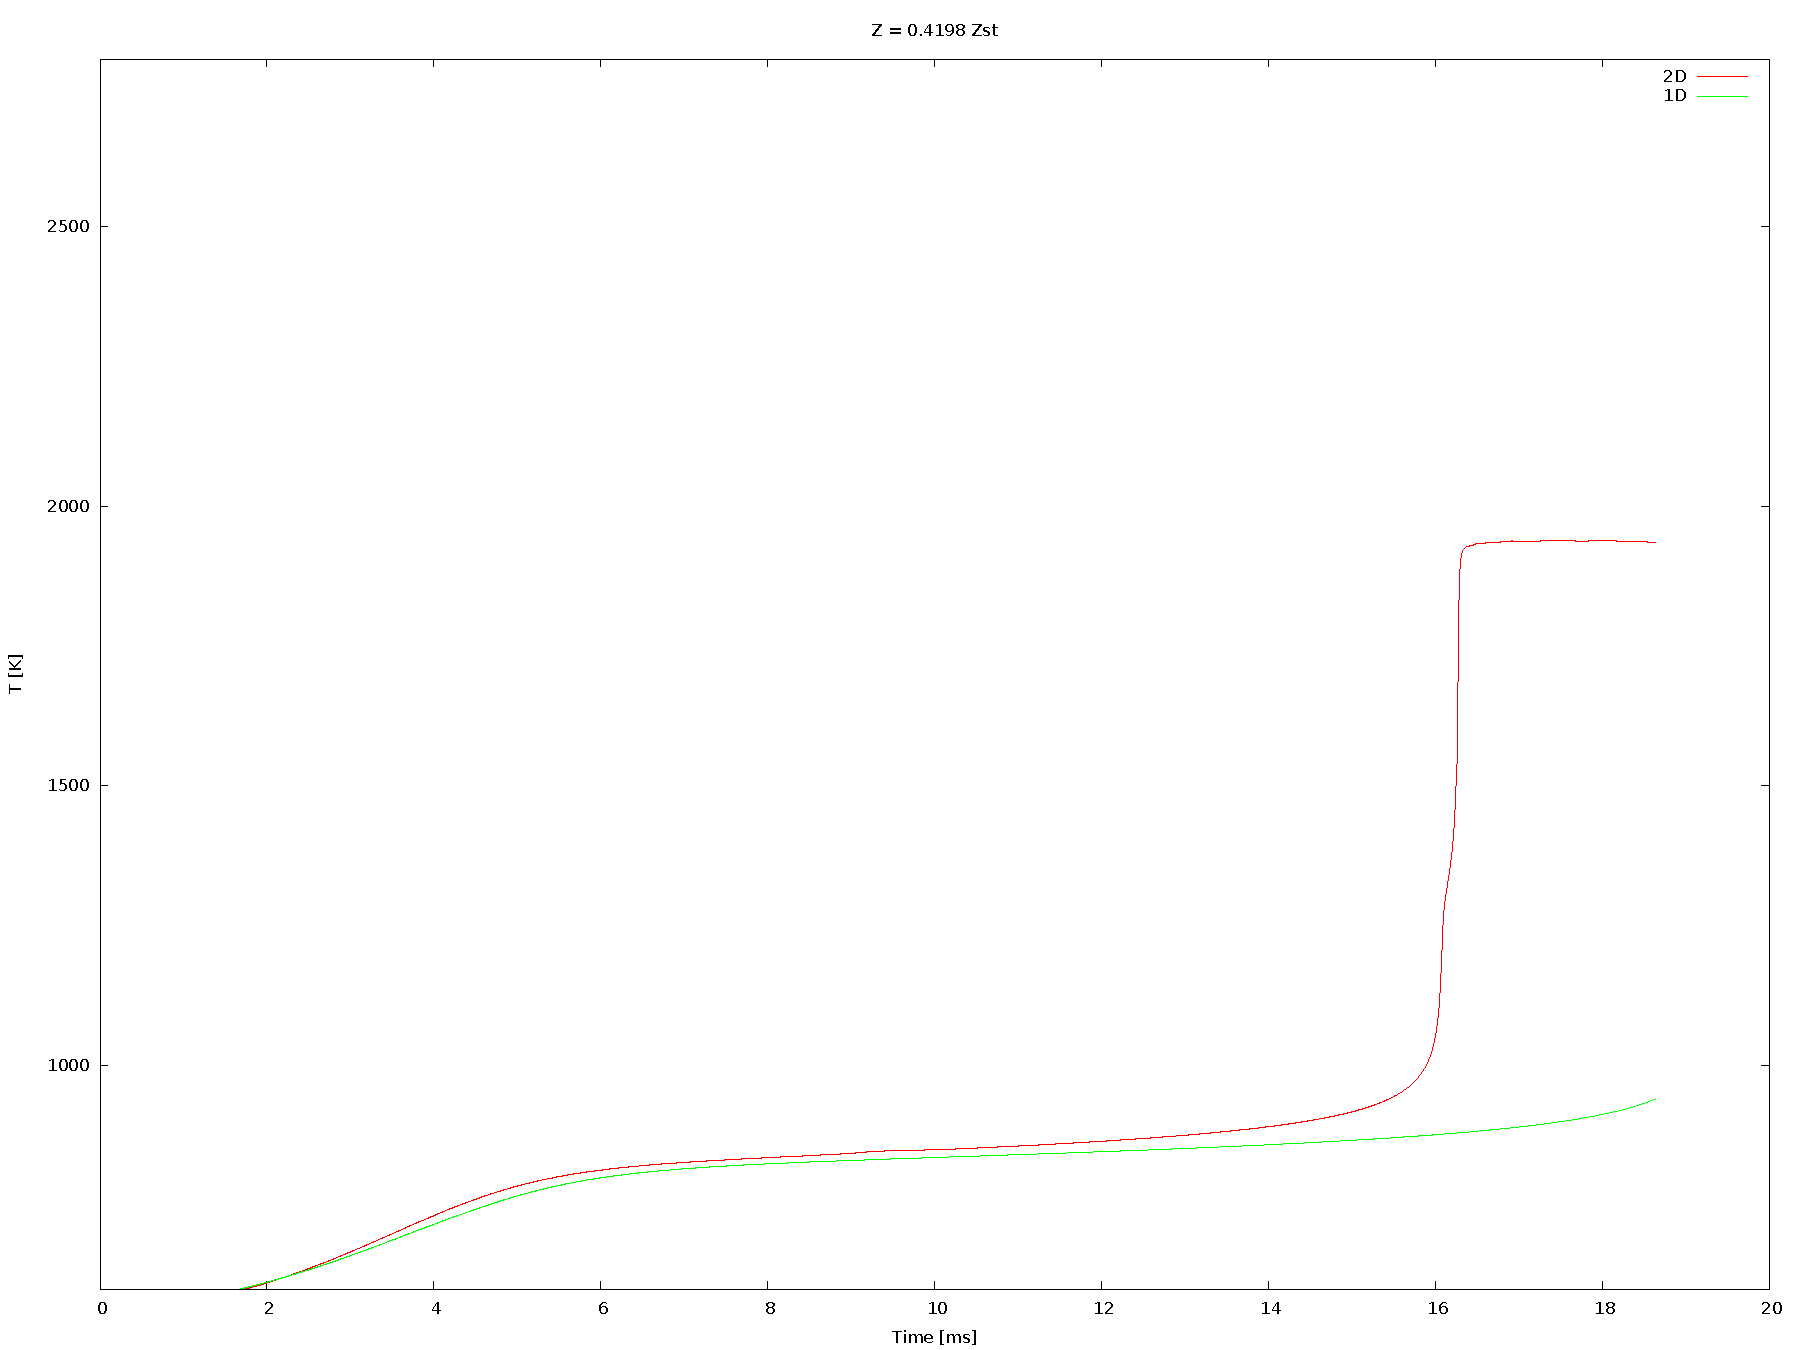
\includegraphics[width=1.0\textwidth]{diluted_800.pdf}
      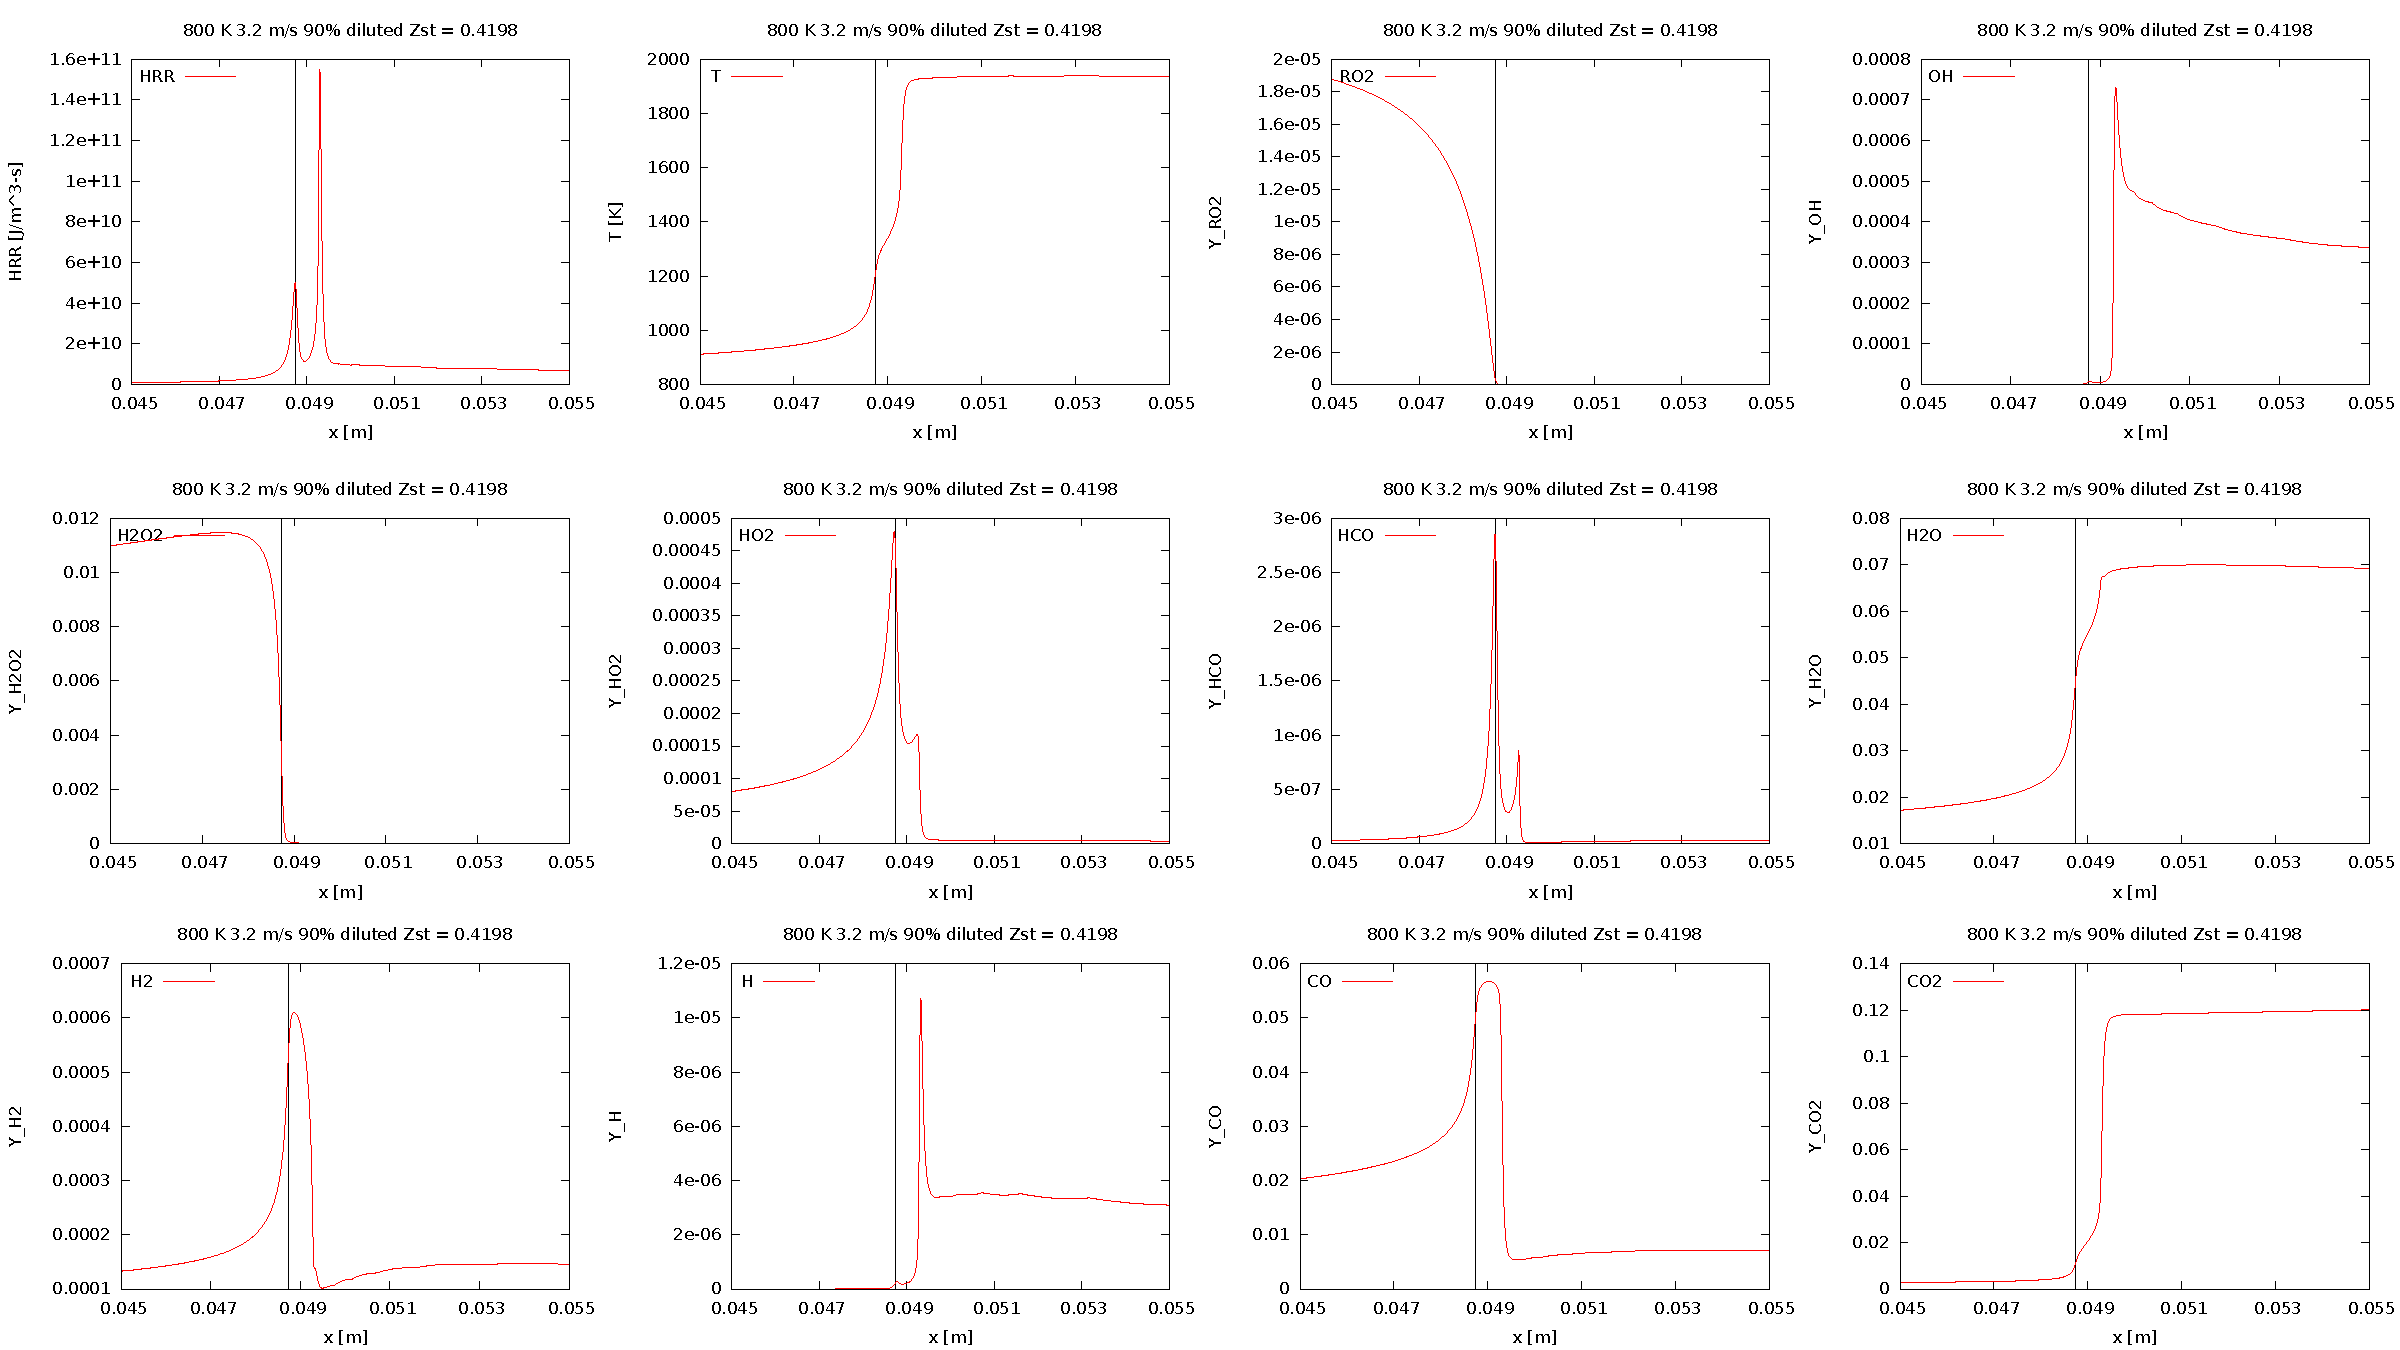
\includegraphics[width=1.0\textwidth]{diluted_800_structure.pdf}
      \normalsize
      %\vspace{-0.1in}
      \caption{With dilution}
      \label{fig:LFA_800_dilution}
    \end{figure} 

%============================================================================
\section{Conclusions}

%============================================================================
\end{document}
